\section{Motivação}

\begin{frame}[fragile]{Motivação}

  \begin{itemize}
    \item Tipos de sessão tradicionais têm inúmeras aplicações
    \newline
  \item Exemplo: Transmitir uma lista num canal de comunicação
    \newline
    
\begin{lstlisting}    
type List = Nil | Cons Int List

type ListServer = &{
  Nil : end
  Cons : ?int . ListServer
}
\end{lstlisting}
  \end{itemize}
\end{frame}


\begin{frame}{Motivação}
  \begin{itemize}
    \item Sequência de operações é definida por um autómato finito:
      \newline
      \usetikzlibrary{automata,positioning}
\tikzstyle{edge} = [draw,thick,->]
\begin{center}
  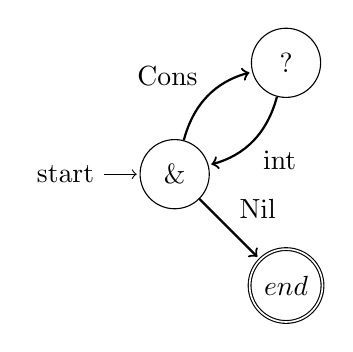
\begin{tikzpicture}[shorten >=1pt,node distance=2cm,on grid,auto] 
   \node[state,initial] (choice)   {$\&$}; 
   \node[state] (input) [above right=of choice] {$?$}; 
   \node[state,accepting] (end) [below right=of choice] {$end$}; 

   \path[edge] (choice) to[bend left] node {Cons} (input);
   \path[edge] (input) to[bend left] node {int} (choice);
   \path[edge] (choice) edge node {Nil} (end);
   
  \end{tikzpicture}
\end{center}

%%% Local Variables:
%%% mode: latex
%%% TeX-master: "cfst-inforum18"
%%% End:
    \item Linguagem regular: $(\textsf{\&Cons}\,\textsf{?Int})^{*}\,\textsf{\&Nil}$
      
  \end{itemize}

\end{frame}

\begin{frame}[fragile]{Motivação}
  \begin{itemize}
  \item E se o objetivo for transmitir uma árvore?
    \newline
    
    \lstinline"type Tree = Leaf | Node Int Tree Tree"
    \newline
  \item Enviar sequências de \lstinline|Node|, \lstinline|Leaf| e \lstinline|Int|\\
    ex: \lstinline|Node Leaf 2 Node Leaf|
  \newline
  \item Comunicação restrita ao envio de tipos básicos e sem passar novos canais
  \newline
  \item Os tipos de sessão devem garantir que as árvores estão bem formadas
  \end{itemize}
\end{frame}

\begin{frame}[fragile]{Motivação}
  \begin{tcolorbox}[colback=blue!5,colframe=blue!60!black,title=Facto,arc=2pt,outer arc=2pt]
    A linguagem produzida pela gramática que descreve um tipo de sessão é:
    \begin{itemize}
    \item Reconhecida por um autómato finito
    \item Uma linguagem ($\omega$-) regular
    \end{itemize}
  \end{tcolorbox}
  \begin{itemize}
  \item \textbf{Gramática:} \lstinline"N ::= Leaf | Node int N N" 
  %\item Linguagem produzida pelo não terminal \lstinline|N| é independente do contexto
  \item \textbf{Consequência:} Os tipos de sessão tradicionais não podem descrever estas estruturas
  \item \textbf{Solução:} Tipos de sessão independentes do contexto propostos por Thiemann e Vasconcelos.
  \end{itemize}
\end{frame}


%%% Local Variables:
%%% mode: latex
%%% TeX-master: "cfst"
%%% End: